% Pore classes for the micromechanics (MMM): from the SCIANTIX state to the MMM runs
% E. Cappellari -- SCIANTIX, technical report for T. Barani, 13 October 2026
% Build: latexmk -pdf mmm_runs.tex      Figures from ../figures/ (python3 ../pore_distribution.py)

\documentclass[10pt,aspectratio=169]{beamer}
\usetheme[progressbar=frametitle,numbering=fraction,block=fill]{metropolis}
\usepackage{amsmath,amssymb,booktabs,graphicx,tikz}
\usetikzlibrary{arrows.meta,positioning}
\usepackage[T1]{fontenc}
\usepackage[utf8]{inputenc}
\graphicspath{{../figures/}}
\definecolor{paper}{RGB}{0,80,180}
\definecolor{own}{RGB}{190,50,40}
\newcommand{\pp}[1]{{\color{paper}#1}}   % from a paper
\newcommand{\oo}[1]{{\color{own}#1}}     % our own choice
\setbeamertemplate{caption}{\raggedright\insertcaption\par}

\title{Pore classes for the micromechanics calcuations}
\subtitle{Input for MMM runs}
\author{E.\ Cappellari}
\institute{Update for T.\ Barani}
\date{13 October 2026}

\begin{document}
\maketitle

% ---------------------------------------------------------------------------------------------------------------------
\begin{frame}{Jernkvist 2019, OperaHPC 5.2: rupture criterion}
\vspace{-4pt}
\[
\oo{\hat s\,\bigl(p-\tfrac{2\gamma}{R}-P_h\bigr)\ \ge\ \sigma_R+P_h}
\quad\Longleftrightarrow\quad
p\ge P_{cr}=P_h+\frac{2\gamma}{R}+\frac{\sigma_R+P_h}{\hat s}
\]
\vspace{6pt}

\begin{columns}[T]
\column{0.49\linewidth}
\pp{Jernkvist 2019} (Olander)
\vspace{4pt}
\[
\pp{P_{cr}=\frac{2\gamma}{R}+\frac{\sigma^{cr}_{hbs}(1-\xi)+P_h}{\xi}},
\]
\vspace{-8pt}
\[
\sigma^{cr}_{hbs}=21\ \text{MPa} \quad \hat s=\frac{\xi}{1-\xi}
\]
\vspace{4pt}
\column{0.49\linewidth}
\pp{OperaHPC D5.2}
\vspace{4pt}
\[
\pp{\sigma_I^{max}\big|_i\ge\sigma_R=275\ \text{MPa}},
\]
\vspace{-8pt}
\[
\hat s_i=\frac{\sigma_I^{max}|_i(1,p_{hyd})+p_{hyd}}{1-p_{hyd}}
\]
\end{columns}
\end{frame}

% ---------------------------------------------------------------------------------------------------------------------
\begin{frame}{Scope and chain of tools}
Goal: replace the mean-field stress factor $\xi/(1-\xi)$ of Jernvist by tables computed with MMM on RVEs that reproduce the pore classes that will be seen by SCIANTIX.
\vspace{6pt}

\centering
\resizebox{\linewidth}{!}{%
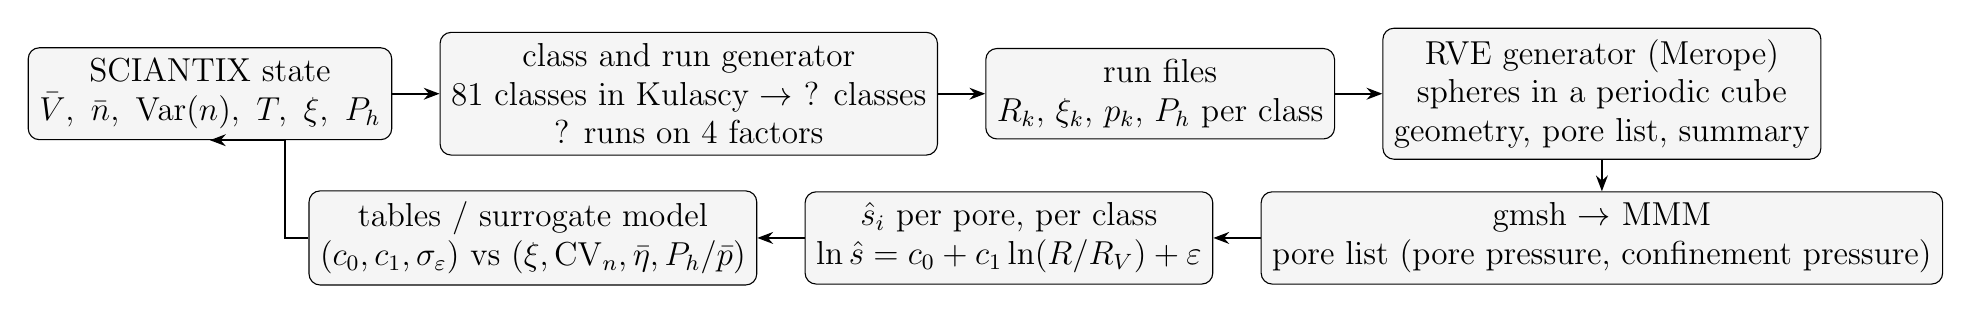
\begin{tikzpicture}[node distance=4mm and 6mm, every node/.style={font=\large},
  box/.style={draw, rounded corners, align=center, minimum height=9mm, inner sep=4pt, fill=black!4},
  arr/.style={-{Stealth[length=2mm]}, thick}]
\node[box] (sx) {SCIANTIX state\\ $\bar V,\ \bar n,\ \mathrm{Var}(n),\ T,\ \xi,\ P_h$};
\node[box, right=of sx] (pd) {class and run generator\\ 81 classes in Kulascy $\to$ ? classes\\ ? runs on 4 factors};
\node[box, right=of pd] (rf) {run files\\ $R_k$, $\xi_k$, $p_k$, $P_h$ per class};
\node[box, right=of rf] (me) {RVE generator (Merope)\\ spheres in a periodic cube\\ geometry, pore list, summary};
\node[box, below=of me] (gm) {gmsh $\to$ MMM \\ pore list (pore pressure, confinement pressure)};
\node[box, left=of gm] (fit) {$\hat s_i$ per pore, per class\\ $\ln\hat s=c_0+c_1\ln(R/R_V)+\varepsilon$};
\node[box, left=of fit] (tab) {tables / surrogate model \\ $(c_0,c_1,\sigma_\varepsilon)$ vs $(\xi,\mathrm{CV}_n,\bar\eta,P_h/\bar p)$};
\draw[arr] (sx) -- (pd); \draw[arr] (pd) -- (rf); \draw[arr] (rf) -- (me); \draw[arr] (me) -- (gm);
\draw[arr] (gm) -- (fit); \draw[arr] (fit) -- (tab); \draw[arr] (tab.west) -| ++(-3mm,0) |- (sx.south);
\end{tikzpicture}}
\end{frame}

% ---------------------------------------------------------------------------------------------------------------------
\begin{frame}{Pore population generator I}
\small
Porosity model from SCIANTIX: $\bar V$ ($R_V$), $\bar n$ = Xe-atoms/pore, $\mathrm{Var}(n)$, $N_p$, $\xi=N_p\bar V$.
\vspace{2pt}
{\footnotesize
\begin{align*}
\pp{\text{log-normal R (K15)}}&:\quad 81\text{ nodes } x_i\in[-4,4],\quad w_i\propto e^{-x_i^2/2},\quad
R_i=R_V\,e^{s x_i}\Big/\bigl(\textstyle\sum_j w_j e^{3 s x_j}\bigr)^{1/3}\ \ (\textstyle\sum_i w_iV_i=\bar V)\\
\oo{\text{Xe/pore distribution}}&:\quad n_i=\bar n\,R_i^{a}\Big/\textstyle\sum_j w_jR_j^{a},\quad a=2\ (\text{gas density}\propto1/R),\qquad
s\ \text{from}\ \textstyle\sum_i w_i(n_i-\bar n)^2=\mathrm{Var}(n)\\
\text{pressure distribution}&:\quad p_i=\frac{n_ik_BT}{V_i}\,Z(\eta_i),\qquad \eta_i=\min\!\Bigl(\frac{n_iv_{Xe}(T)}{V_i},0.65\Bigr)\quad\text{hard spheres}
\end{align*}}
\vspace{-8pt}
\centering\includegraphics[width=\linewidth]{classes_distributions.png}

\scriptsize NFIR, end of base irradiation: $s=0.33$ (measured about 0.3, K15 0.356), radii 0.08--1.1 $\mu$m, $p_i$ from 2.7 GPa to 30 MPa.
\end{frame}

% ---------------------------------------------------------------------------------------------------------------------
\begin{frame}{Pore population generator II}
\small
\begin{align*}
\sum_iw_iV_i&=\bar V && \text{exact by construction}\\
\sum_iw_in_i&=\bar n && \text{exact by construction}\\
\mathrm{CV}_n^2(s,a)&=\frac{\sum_iw_ie^{2asx_i}}{\bigl(\sum_iw_ie^{asx_i}\bigr)^2}-1=\frac{\mathrm{Var}(n)}{\bar n^2} && \text{root in }s
\end{align*}
Mean pressure (pressure of the volume-weighted density): $p_{EoS}(\bar n,\bar V,T)$ is conserved. 

\centering\includegraphics[width=0.9\linewidth]{classes_moment_errors.png}
\end{frame}

% ---------------------------------------------------------------------------------------------------------------------
\begin{frame}{Pore population generator III: Xe atoms/pore}
\includegraphics[width=0.4\textwidth]{classes_closure_exponent.png}
\includegraphics[width=0.59\textwidth]{classes_heatup.png}
\vspace{2pt}
\centering
The moments hold for every $a$; what changes is the width $s$, the pressure spread and which classes break: small pores first for $a<3$, while for $a=3$ uniform pressure.
\end{frame}

% ---------------------------------------------------------------------------------------------------------------------
\begin{frame}{Reduction of the parameter space}
\small
MMM calculations will be scale-free and linear in the load: $R_V$ and $\bar p$ only set the scale. With $p^*=p\,v_{Xe}/k_BT$ the EoS has no explicit $T$,
\[
p_i^*=\eta_iZ(\eta_i),\qquad \bar\eta=\frac{\bar n\,v_{Xe}(T)}{\bar V},\qquad \mathrm{CV}_n=\frac{\sqrt{\mathrm{Var}(n)}}{\bar n}
\]
so in $x_i=R_i/R_V$ the shape $p_i/\bar p$ and the weights $w_i$ depend on $(\bar\eta,\mathrm{CV}_n,a)$ only.
\vspace{4pt}

\centering
\begin{tabular}{@{}ll@{}}
\toprule
factor & sets  \\
\midrule
$\xi$ & porosity, pore distances \\
$s$ (from $\mathrm{CV}_n$) & $R_k/R_V$ and the shares $\xi_k/\xi$ \\
$\bar\eta$ & with $s$, the pressure profile $p_k/\bar p$  \\
$P_h/\bar p$ & net load $p_k-P_h$ of every class \\
\bottomrule
\end{tabular}

How to cover the parameter space for Merope + MMM run? 
Ranges and levels to be defined, LHS could be a way to define the different combinations.
\end{frame}

% ---------------------------------------------------------------------------------------------------------------------
\begin{frame}{Parameter influence}
\centering\includegraphics[width=\linewidth]{classes_coverage.png}
\end{frame}

% ---------------------------------------------------------------------------------------------------------------------
\begin{frame}{Merope}

For every run file:
\begin{enumerate}
\item read the 4 columns, sort the classes by decreasing radius, check that $P_h$ is one value
\item expected pores per class $=\xi_k/V_k\cdot L^3$
\item throw the spheres by RSA in a periodic cube, one (radius, porosity) pair per class, with a repulsion distance
\item each sphere gets the class with the nearest radius, hence its pressure; one phase id per sphere, not meshed
\item write, in one folder per run, seed and repulsion: the pore list (id, $x,y,z$, $R$, $p$), a summary (obtained vs asked porosity per class, pore counts), the geometry for gmsh
\end{enumerate}

\centering
Fixed in the generator:\\[2pt]
\begin{tabular}{@{}lll@{}}
\toprule
cube & 30 $\mu$m & $\approx86\,R_V$\\
repulsion & 0.3 $\mu$m & to verify a posteriori\\
mesh & 0.15 $\mu$m & $>R_{min}/2$, to be checked\\
seed & 5 & \\
\bottomrule
\end{tabular}

\end{frame}

% ---------------------------------------------------------------------------------------------------------------------
\begin{frame}{Status}
\footnotesize
\begin{itemize}
\item Xe atoms / pore - distribution is fixed by a.
\item Dislocation punching pressure.
\item LHS sampling and parameter range.
\item Pore count (smallest class should be represented).
\item Smallest classes should be resolved,by the mesh size.
\item Repulsion distance should scale with the radius?
\item 1 seed per run.
\item Merope + MMM calculations on few runs to evaluate computational cost.
\item Surrogate model: training (LHS sampling) and validation dataset (additional cases). 
\end{itemize}
\end{frame}

% ---------------------------------------------------------------------------------------------------------------------
\begin{frame}{Other stuff}
\small
\begin{itemize}
\item \textbf{Form for Marjorie}: filled in; to confirm the affiliation to put (PLEIADES or UT) and the phone number field.
\item \textbf{Abstract}: review requested before submission.
\item \textbf{Lectures}: indicative dates of absence 3--5 November.
\item \textbf{Transparant online meeting at the end of the month}: I would ask for a day off this week, working from home for the meeting.
\end{itemize}
\end{frame}

\end{document}
